\documentclass{article}\usepackage[]{graphicx}\usepackage[]{color}
%% maxwidth is the original width if it is less than linewidth
%% otherwise use linewidth (to make sure the graphics do not exceed the margin)
\makeatletter
\def\maxwidth{ %
  \ifdim\Gin@nat@width>\linewidth
    \linewidth
  \else
    \Gin@nat@width
  \fi
}
\makeatother

\definecolor{fgcolor}{rgb}{0.345, 0.345, 0.345}
\newcommand{\hlnum}[1]{\textcolor[rgb]{0.686,0.059,0.569}{#1}}%
\newcommand{\hlstr}[1]{\textcolor[rgb]{0.192,0.494,0.8}{#1}}%
\newcommand{\hlcom}[1]{\textcolor[rgb]{0.678,0.584,0.686}{\textit{#1}}}%
\newcommand{\hlopt}[1]{\textcolor[rgb]{0,0,0}{#1}}%
\newcommand{\hlstd}[1]{\textcolor[rgb]{0.345,0.345,0.345}{#1}}%
\newcommand{\hlkwa}[1]{\textcolor[rgb]{0.161,0.373,0.58}{\textbf{#1}}}%
\newcommand{\hlkwb}[1]{\textcolor[rgb]{0.69,0.353,0.396}{#1}}%
\newcommand{\hlkwc}[1]{\textcolor[rgb]{0.333,0.667,0.333}{#1}}%
\newcommand{\hlkwd}[1]{\textcolor[rgb]{0.737,0.353,0.396}{\textbf{#1}}}%

\usepackage{framed}
\makeatletter
\newenvironment{kframe}{%
 \def\at@end@of@kframe{}%
 \ifinner\ifhmode%
  \def\at@end@of@kframe{\end{minipage}}%
  \begin{minipage}{\columnwidth}%
 \fi\fi%
 \def\FrameCommand##1{\hskip\@totalleftmargin \hskip-\fboxsep
 \colorbox{shadecolor}{##1}\hskip-\fboxsep
     % There is no \\@totalrightmargin, so:
     \hskip-\linewidth \hskip-\@totalleftmargin \hskip\columnwidth}%
 \MakeFramed {\advance\hsize-\width
   \@totalleftmargin\z@ \linewidth\hsize
   \@setminipage}}%
 {\par\unskip\endMakeFramed%
 \at@end@of@kframe}
\makeatother

\definecolor{shadecolor}{rgb}{.97, .97, .97}
\definecolor{messagecolor}{rgb}{0, 0, 0}
\definecolor{warningcolor}{rgb}{1, 0, 1}
\definecolor{errorcolor}{rgb}{1, 0, 0}
\newenvironment{knitrout}{}{} % an empty environment to be redefined in TeX

\usepackage{alltt}

%\VignetteEngine{knitr::knitr}
%\VignetteIndexEntry{qvalue Package}

\usepackage{graphics}
\usepackage{amsmath}
\usepackage{fullpage}
\usepackage{bibentry}
\usepackage[parfill]{parskip}
\setlength{\parskip}{10pt}
%\usepackage{indentfirst}
\usepackage[colorlinks=true]{hyperref}
\usepackage[utf8]{inputenc}
\nobibliography*
\IfFileExists{upquote.sty}{\usepackage{upquote}}{}
\begin{document}



\title{Bioconductor's {\tt edge} package \\ Version 0.99.0}
\author{John D. Storey and Andrew J. Bass \\ Princeton University \\ \url{http://genomine.org/contact.html}}
\maketitle
\tableofcontents
\newpage
\section{Introduction}

{\tt edge} is an open-source software package for significance analysis of DNA microarray experiments, and is able  to identify genes that are differentially expressed between two or more different biological conditions (e.g., healthy versus diseased tissue). There are a number of existing software packages to perform significance analysis but {\tt edge} uses the odp-statistic from the Optimal Discovery Procedure (ODP). Whereas previously existing methods employ statistics that are essentially designed for testing one gene at a time (e.g., t-statistics and F-statistics), the ODP uses information across all genes to test for differential expression. 

The improvements in power are substantial; Figure 1 shows a comparison between edge and five leading software packages, based on a well-known breast cancer expression study (Hedenfalk et al. 2001). In addition to the significance analysis procedures for identifying differentially expressed genes, {\tt edge} includes implementations of popular packages such as {\tt snm}, {\tt sva}, {\tt qvalue} and {\tt ExpressionSet}. 

\begin{figure}[ht]
\begin{center}
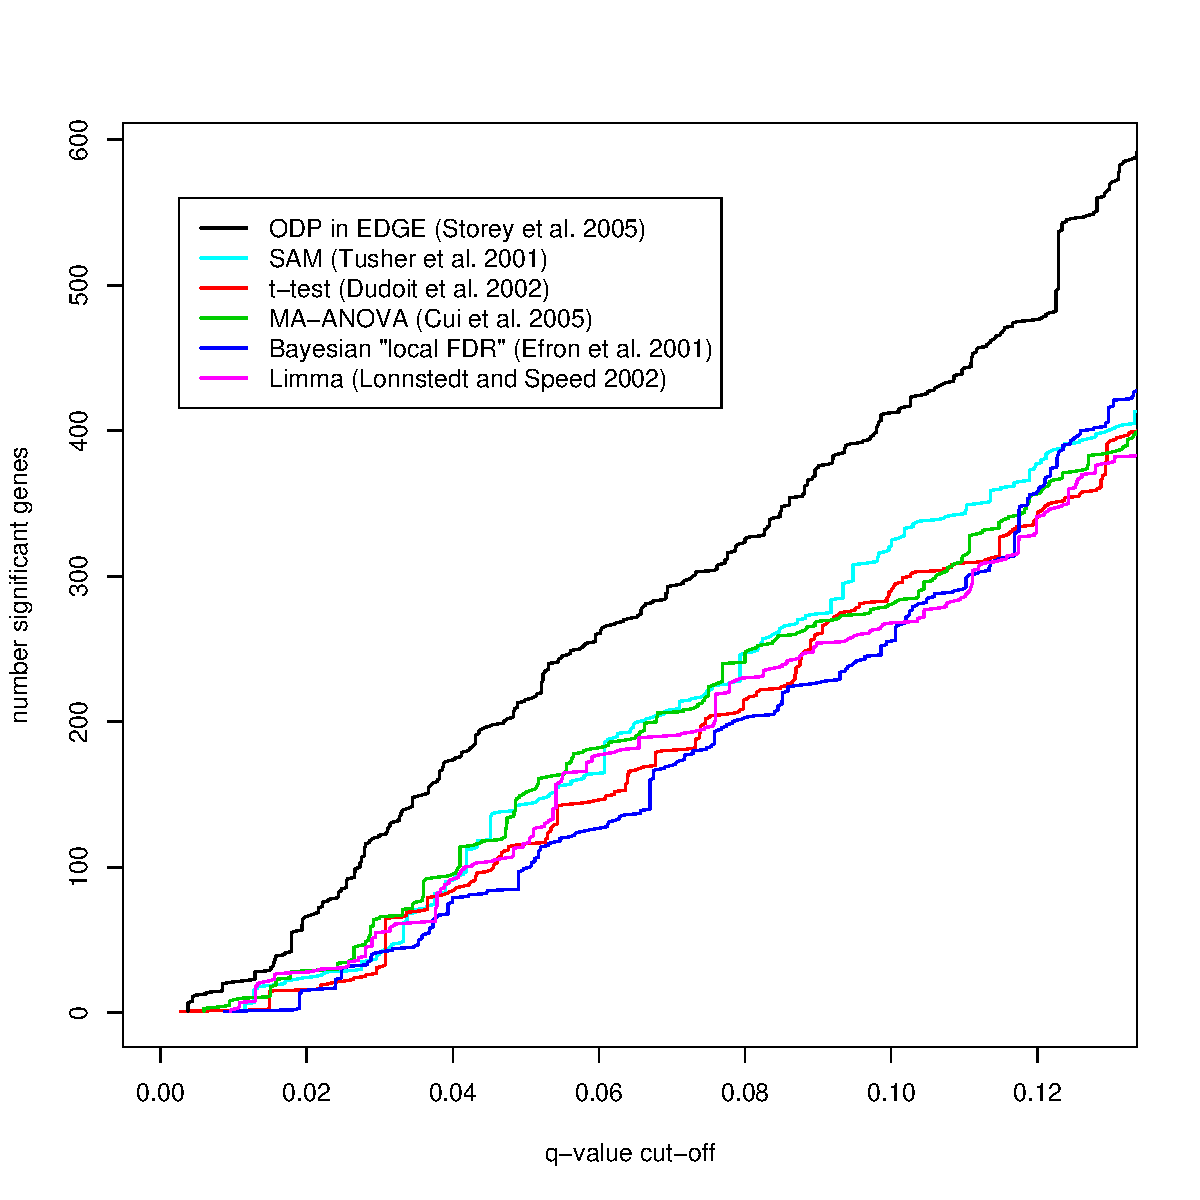
\includegraphics[scale=.50]{edgecomp.pdf}
\end{center}
\caption{Comparison of EDGE to various other leading methods for identifying differential expressed genes in the Hedenfalk et al., 2001 study. Figure retrieved from Leek et al. (2005).}
\label{fig:test}
\end{figure}

%There are three experimental designs where {\tt edge} can identify differentially expressed genes: static, time course and continuous response experiments. In a ``static sampling'' experiment, the arrays have been collected from distinct biological groups without respect to time. The goal is to identify genes that have a statistically significant difference in average expression across these distinct biological groups. The second type of experiment is a time course experiment, where the arrays have been sampled with respect to time from one or more distinct biological groups. If only one biological group has been sampled, then the goal is to identify genes that show ``within-class temporal differential expression'', i.e., genes that show statistically significant changes in expression over time. If two or more biological groups have been sampled, then the goal is to identify genes that show ``between-class temporal differential expression'', i.e., genes that show statistically significant differences in expression over time between the various groups. The third type of experiment is a ``continuous response'' design, which means that the arrays have been collected from a continuously defined biological state without respect to time. The goal here is to identify genes whose expression shows a statistically significant change with respect to this continuous response.
%\texttt{edge} uses methods that have been specifically designed for time course experiments because many things can go wrong when using traditional static analysis for time course experiments. Even though some significance analysis packages allow for users to enter information about time points, we have a rigorously developed set of methodology that was published in Storey et al. (2005b) that simplifies the process for time course experiments. All procedures implemented in the software are based on proven statistical procedures that have appeared in peer-reviewed articles. 

%An important statistical quantity of interest that {\tt edge} returns is the q-value. The q-value is like the p-value, except designed for false discovery rates: a gene's q-value gives the false discovery rate that is incurred when calling that gene significant. The q-values are estimated using the methodology presented in Storey (2002) and Storey \& Tibshirani (2003). See the documentation on {\tt qvalue} for more information. A manual on q-value estimation is available at \url{http://genomics.princeton.edu/storeylab/qvalue/}.
\section{Citing this package}

\bibentry{storey:2007}.

\bibentry{storey:etal:2007}.

\bibentry{woo:leek:storey:2011}.

\section{Getting help}
Hopefully most questions relating to the package will be answered in the vignette but to get a more detailed account of how to use the functions simply type, within R:
\begin{knitrout}
\definecolor{shadecolor}{rgb}{0.969, 0.969, 0.969}\color{fgcolor}\begin{kframe}
\begin{alltt}
\hlkwd{help}\hlstd{(}\hlkwc{package} \hlstd{=} \hlstr{"edge"}\hlstd{)}
\end{alltt}
\end{kframe}
\end{knitrout}
\noindent Please contact the authors directly with any issues regarding bugs. Otherwise, any questions or problems implementing {\tt edge} will most efficiently be addressed on the Bioconductor mailing list, \url{http://stat.ethz.ch/mailman/listinfo/bioconductor}.

\section{Quick start guide}
There are two ways to use {\tt edge}: (i) using {\tt edgeModel} or (ii) using an {\tt ExpressionSet} object. Using {\tt edgeModel} has less flexibility and is designed to help users create alternative and null models from their experiment.

An example of using {\tt edgeModel} for significance analysis:
\begin{knitrout}
\definecolor{shadecolor}{rgb}{0.969, 0.969, 0.969}\color{fgcolor}\begin{kframe}
\begin{alltt}
\hlcom{# Import data}
\hlkwd{data}\hlstd{(kidney)}
\hlstd{sex} \hlkwb{<-} \hlstd{kidney}\hlopt{$}\hlstd{sex[kidney}\hlopt{$}\hlstd{tissue} \hlopt{==} \hlstr{"c"}\hlstd{]}
\hlstd{age} \hlkwb{<-} \hlstd{kidney}\hlopt{$}\hlstd{age[kidney}\hlopt{$}\hlstd{tissue} \hlopt{==} \hlstr{"c"}\hlstd{]}
\hlstd{kidexpr} \hlkwb{<-} \hlkwd{log}\hlstd{(kidney}\hlopt{$}\hlstd{kidexpr[, kidney}\hlopt{$}\hlstd{tissue} \hlopt{==}
    \hlstr{"c"}\hlstd{]} \hlopt{+} \hlnum{10}\hlstd{)}

\hlcom{# Create edgeSet object from edgeModel}
\hlstd{edgeObj} \hlkwb{<-} \hlkwd{edgeModel}\hlstd{(}\hlkwc{data} \hlstd{= kidexpr,} \hlkwc{adj.var} \hlstd{=} \hlkwd{model.matrix}\hlstd{(}\hlopt{~}\hlstd{sex),}
    \hlkwc{tme} \hlstd{= age,} \hlkwc{sampling} \hlstd{=} \hlstr{"timecourse"}\hlstd{,} \hlkwc{basis.df} \hlstd{=} \hlnum{4}\hlstd{)}

\hlcom{# Optimal Discovery Procedure}
\hlstd{edgeODP} \hlkwb{<-} \hlkwd{odp}\hlstd{(edgeObj)}

\hlcom{# Likelihood Ratio Test}
\hlstd{edgeLRT} \hlkwb{<-} \hlkwd{lrt}\hlstd{(edgeObj)}
\end{alltt}
\end{kframe}
\end{knitrout}

Given an {\tt ExpressionSet} object and both the alternative and null hypothesis, the {\tt odp} or {\tt lrt} function can be used as follows:


\begin{knitrout}
\definecolor{shadecolor}{rgb}{0.969, 0.969, 0.969}\color{fgcolor}\begin{kframe}
\begin{alltt}
\hlcom{# Create ExpressionSet}
\hlstd{expSet} \hlkwb{<-} \hlkwd{ExpressionSet}\hlstd{(}\hlkwc{assayData} \hlstd{= kidexpr,} \hlkwc{phenoData} \hlstd{=} \hlkwd{as}\hlstd{(}\hlkwd{data.frame}\hlstd{(}\hlkwc{sex} \hlstd{= sex,}
    \hlkwc{age} \hlstd{= age),} \hlstr{"AnnotatedDataFrame"}\hlstd{))}

\hlcom{# Create Models}
\hlstd{nModel} \hlkwb{<-} \hlopt{~}\hlstd{sex}
\hlstd{fModel} \hlkwb{<-} \hlopt{~}\hlstd{sex} \hlopt{+} \hlkwd{ns}\hlstd{(age,} \hlkwc{df} \hlstd{=} \hlnum{3}\hlstd{,} \hlkwc{intercept} \hlstd{=} \hlnum{FALSE}\hlstd{)}

\hlcom{# Create edgeSet object from ExpressionSet object}
\hlstd{edgeObj} \hlkwb{<-} \hlkwd{edgeSet}\hlstd{(expSet,} \hlkwc{full.model} \hlstd{= fModel,} \hlkwc{null.model} \hlstd{= nModel)}

\hlcom{# Optimal Discovery Procedure}
\hlstd{edgeODP} \hlkwb{<-} \hlkwd{odp}\hlstd{(edgeObj)}

\hlcom{# Likelihood Ratio Test}
\hlstd{edgeLRT} \hlkwb{<-} \hlkwd{lrt}\hlstd{(edgeObj)}
\end{alltt}
\end{kframe}
\end{knitrout}

In the above models, {\tt fModel} is the alternative hypothesis and {\tt nModel} is the null hypothesis. It is recommended to create an {\tt ExpressionSet} object because of the flexibility in creating the null and alternative hypothesis. The following sections of the manual go through a case study to show additional features of the {\tt edge} package.

\section{Examples}
Three different examples will be used to show the functionality of {\tt edge}. 
In each example, there will be a different type of experiment: static, longitudinal and independent. It will become evident that in each case, the process is very similar and the only step that differs is the model setup.

The three main steps when using {\tt edge}:
\begin{itemize}
\item Write the alternative and null models of the experiment. In this manual they will be called {\tt altMod} and {\tt nullMod}. 
\item Use an {\tt ExpressionSet} object to create an {\tt edgeSet} object by using function {\tt edgeSet}. 
\item Either use {\tt edgeFit} to extract the fitted values, residuals and/or coefficients from both models or run functions {\tt odp}/{\tt lrt} directly to obtain the q-value object. See {\tt ?qvalue}.
\end{itemize}

\subsection{Creating the models}
The example datasets in this section each represent different experimental designs: the kidney dataset is an independent time course design, the endotoxin dataset is a longitudinal time course study and the gibson dataset is a static experiment. We will go through each case to show how hypothesis tests are setup in {\tt edge}. 

\paragraph{Kidney dataset} Gene expression measurements from kidney samples were obtained from 72 human subjects ranging in age from 27 to 92 years. Only one array was obtained per sample, the age and tissue type of each subject was recorded. There are two covariates in this dataset: sex and age. We are interested in finding the effect of age on gene expression. In this case, we handle the time variable, age, by fitting a natural spline curve as presented by Storey (2005).  

\begin{knitrout}
\definecolor{shadecolor}{rgb}{0.969, 0.969, 0.969}\color{fgcolor}\begin{kframe}
\begin{alltt}
\hlstd{nullMod} \hlkwb{<-} \hlopt{~-}\hlnum{1} \hlopt{+} \hlkwd{as.factor}\hlstd{(sex)}
\hlstd{altMod} \hlkwb{<-} \hlopt{~-}\hlnum{1} \hlopt{+} \hlkwd{as.factor}\hlstd{(sex)} \hlopt{+} \hlkwd{ns}\hlstd{(age,} \hlkwc{df} \hlstd{=} \hlnum{4}\hlstd{)}
\end{alltt}
\end{kframe}
\end{knitrout}

\paragraph{Endotoxin dataset} The endotoxin dataset provide gene expression measurements in an endotoxin study where four subjects were given endotoxin and four subjects were given a placebo. Blood samples were collected and leukocytes were isolated from the samples before infusion and measurement were recorded at times 2, 4, 6, 9, 24 hours. We are interested in identifying genes that vary over time between the endotoxin and control groups. In this example, the models are slightly more complicated. The two covariates are time and class. For the null model we fit a spline curve for the time variable and the full model will contain the class variable and an interaction term between class and time. 

\begin{knitrout}
\definecolor{shadecolor}{rgb}{0.969, 0.969, 0.969}\color{fgcolor}\begin{kframe}
\begin{alltt}
\hlstd{mNull} \hlkwb{<-} \hlopt{~-}\hlnum{1} \hlopt{+} \hlkwd{ns}\hlstd{(time,} \hlkwc{df} \hlstd{=} \hlnum{4}\hlstd{,} \hlkwc{intercept} \hlstd{=} \hlnum{FALSE}\hlstd{)}
\hlstd{mFull} \hlkwb{<-} \hlopt{~-}\hlnum{1} \hlopt{+} \hlkwd{ns}\hlstd{(time,} \hlkwc{df} \hlstd{=} \hlnum{4}\hlstd{,} \hlkwc{intercept} \hlstd{=} \hlnum{FALSE}\hlstd{)} \hlopt{+}
    \hlkwd{ns}\hlstd{(time,} \hlkwc{df} \hlstd{=} \hlnum{4}\hlstd{,} \hlkwc{intercept} \hlstd{=} \hlnum{FALSE}\hlstd{)}\hlopt{:}\hlstd{class} \hlopt{+} \hlstd{class}
\end{alltt}
\end{kframe}
\end{knitrout}

\paragraph{Gibson dataset} The gibson dataset provides gene expression measurements in peripheral blood leukocyte samples from three Moroccan Amazigh groups leading distinct ways of life: desert nomadic (DESERT), mountain agrarian (VILLAGE), and coastal urban (AGADIR). Suppose we are interested in finding the genes that differentiate the Moroccan Amazigh groups the most. There are three covariates in this dataset: Gender, Batch and Location. Since we are interested in finding the genes that differentiate the three groups the most, the variable Location will be included in the alternative model.

\begin{knitrout}
\definecolor{shadecolor}{rgb}{0.969, 0.969, 0.969}\color{fgcolor}\begin{kframe}
\begin{alltt}
\hlstd{nullMod} \hlkwb{<-} \hlopt{~}\hlstd{Gender} \hlopt{+} \hlstd{Batch}
\hlstd{altMod} \hlkwb{<-} \hlopt{~}\hlstd{Gender} \hlopt{+} \hlstd{Batch} \hlopt{+} \hlstd{Location}
\end{alltt}
\end{kframe}
\end{knitrout}
 
 
\subsection{\texttt{edgeSet} object}
The {\tt edgeSet} object is the main class for {\tt edge}. The {\tt edgeSet} object contains q-value information among other experimental data inherited from the {\tt ExpressionSet}. The {\tt edgeSet} function requires an {\tt ExpressionSet} object. To create an {\tt ExpressionSet} using the {\tt kidney} dataset as an example:
\begin{knitrout}
\definecolor{shadecolor}{rgb}{0.969, 0.969, 0.969}\color{fgcolor}\begin{kframe}
\begin{alltt}
\hlkwd{library}\hlstd{(edge)}
\hlkwd{data}\hlstd{(kidney)}

\hlcom{# Interested in cortex samples }
\hlstd{sex} \hlkwb{<-} \hlstd{kidney}\hlopt{$}\hlstd{sex[kidney}\hlopt{$}\hlstd{tissue}\hlopt{==}\hlstr{"c"}\hlstd{]}
\hlstd{age} \hlkwb{<-} \hlstd{kidney}\hlopt{$}\hlstd{age[kidney}\hlopt{$}\hlstd{tissue}\hlopt{==}\hlstr{"c"}\hlstd{]}
\hlstd{kidexpr} \hlkwb{<-} \hlstd{kidney}\hlopt{$}\hlstd{kidexpr[, kidney}\hlopt{$}\hlstd{tissue}\hlopt{==}\hlstr{"c"}\hlstd{]}
\hlstd{expSet} \hlkwb{<-} \hlkwd{ExpressionSet}\hlstd{(}\hlkwc{assayData} \hlstd{= kidexpr,}
                        \hlkwc{phenoData} \hlstd{=} \hlkwd{as}\hlstd{(}\hlkwd{data.frame}\hlstd{(}\hlkwc{age}\hlstd{=age,} \hlkwc{sex}\hlstd{=sex),} \hlstr{"AnnotatedDataFrame"}\hlstd{))}
\end{alltt}
\end{kframe}
\end{knitrout}
To access the expression values, one can use the function {\tt exprs(expSet)} or to access the covariates, {\tt pData(expSet)}. The {\tt ExpressionSet} class is a widely used object in Bioconductor and more information can be found \url{http://www.bioconductor.org/packages/2.14/bioc/html/Biobase.html}. 


Using the {\tt ExpressionSet} object to create an {\tt edgeSet} is very simple once the alternative and null models are known: 
\begin{knitrout}
\definecolor{shadecolor}{rgb}{0.969, 0.969, 0.969}\color{fgcolor}\begin{kframe}
\begin{alltt}
\hlcom{# null and full models}
\hlstd{nullMod} \hlkwb{<-} \hlopt{~-}\hlnum{1} \hlopt{+} \hlkwd{as.factor}\hlstd{(sex)}
\hlstd{altMod} \hlkwb{<-} \hlopt{~-}\hlnum{1} \hlopt{+} \hlkwd{as.factor}\hlstd{(sex)} \hlopt{+} \hlkwd{ns}\hlstd{(age,} \hlkwc{df} \hlstd{=} \hlnum{4}\hlstd{)}
\hlstd{edgeObj} \hlkwb{<-} \hlkwd{edgeSet}\hlstd{(expSet,} \hlkwc{full.model} \hlstd{= altMod,} \hlkwc{null.model} \hlstd{= nullMod)}
\end{alltt}
\end{kframe}
\end{knitrout}

The object contains the following slots:
\begin{itemize}
\item {\tt full.model}: the full model of the experiment
\item {\tt null.model}: the null model of the experiment
\item {\tt full.matrix}: the full model in matrix form
\item {\tt null.matrix}: the null model in matrix form
\item {\tt individual}: containing information on individuals in the experiment
\item {\tt qvalue.obj}: {\tt qvalue} list
\item {\tt ExpressionSet}- inherits the slots from {\tt ExpressionSet} object
\end{itemize}
The qvalue information can be accessed from the object by using {\tt qvalue.obj(object)}. See {\tt ?edgeSet} for more details on how to extract and set each slot in the object.

\subsection{edgeFit}

The {\tt edgeFit} contains information on the model fitting phase of the procedure. The slots for the object are
\begin{itemize}
\item fit.full- fitted values for full model
\item fit.null- fitted values for null model
\item res.full- residuals for the full model
\item res.null- residuals for the null models
\item dH.full- diaganol elements in the projection matrix for the full model
\item beta.coef- the coefficients for the full model
\item stat.type- statistic type used, either "odp" or "lrt"
\end{itemize}
To access the coefficients in the {\tt edgeFit} object, the user only has to type {\tt beta.coef(object)}. Similarly, to access the full residuals, {\tt fit.full(object)}.

\section{Static study: {\tt gibson} dataset}
Lets begin the analysis by importing the data and creating an \texttt{ExpressionSet},

\begin{knitrout}
\definecolor{shadecolor}{rgb}{0.969, 0.969, 0.969}\color{fgcolor}\begin{kframe}
\begin{alltt}
\hlkwd{library}\hlstd{(edge)}
\hlkwd{data}\hlstd{(gibson)}
\hlstd{covar} \hlkwb{<-} \hlkwd{data.frame}\hlstd{(}\hlkwd{t}\hlstd{(gibson}\hlopt{$}\hlstd{covar))}
\hlstd{expSet} \hlkwb{<-} \hlkwd{ExpressionSet}\hlstd{(}\hlkwc{assayData}\hlstd{=gibson}\hlopt{$}\hlstd{exprdat,}
                        \hlkwc{phenoData}\hlstd{=}\hlkwd{as}\hlstd{(covar,} \hlstr{"AnnotatedDataFrame"}\hlstd{))}
\end{alltt}
\end{kframe}
\end{knitrout}

The next step is to determine the model equations for the experiment. Note that the alternative model must include the null model in its formulation. In this example, there are the covariates {\tt Gender}, {\tt Batch} and {\tt Location}. The {\tt Gender} and {\tt Batch} covariates are the adjustment variables and the {\tt Location} is the biological variable. The models will look like

\begin{knitrout}
\definecolor{shadecolor}{rgb}{0.969, 0.969, 0.969}\color{fgcolor}\begin{kframe}
\begin{alltt}
\hlstd{nullMod} \hlkwb{<-} \hlopt{~}\hlstd{Gender} \hlopt{+} \hlstd{Batch}
\hlstd{altMod} \hlkwb{<-} \hlopt{~}\hlstd{Gender} \hlopt{+} \hlstd{Batch} \hlopt{+} \hlstd{Location}
\hlstd{edgeObj} \hlkwb{<-} \hlkwd{edgeSet}\hlstd{(expSet,} \hlkwc{full.model} \hlstd{= altMod,} \hlkwc{null.model} \hlstd{= nullMod)}
\end{alltt}
\end{kframe}
\end{knitrout}

The function {\tt edgeFit} can be used to retrieve the fitted values of the model. See {\tt ?edgeFit} for more details. To run {\tt odp} or {\tt lrt} on the dataset to identify differentially expression genes,

\begin{knitrout}
\definecolor{shadecolor}{rgb}{0.969, 0.969, 0.969}\color{fgcolor}\begin{kframe}
\begin{alltt}
\hlstd{edge.odp} \hlkwb{<-} \hlkwd{odp}\hlstd{(edgeObj,} \hlkwc{bs.its}\hlstd{=}\hlnum{100}\hlstd{,} \hlkwc{verbose}\hlstd{=}\hlnum{FALSE}\hlstd{)}
\hlstd{edge.lrt} \hlkwb{<-} \hlkwd{lrt}\hlstd{(edgeObj,} \hlkwc{nullDistn}\hlstd{=}\hlstr{"normal"}\hlstd{)}
\end{alltt}


{\ttfamily\noindent\bfseries\color{errorcolor}{\#\# Error: could not find function "{}lrtStat"{}}}\end{kframe}
\end{knitrout}

Comparing the findings between both methods:
\begin{knitrout}
\definecolor{shadecolor}{rgb}{0.969, 0.969, 0.969}\color{fgcolor}\begin{kframe}
\begin{alltt}
\hlkwd{plot}\hlstd{(}\hlkwd{qvalue.obj}\hlstd{(edge.odp))}
\end{alltt}
\end{kframe}

{\centering 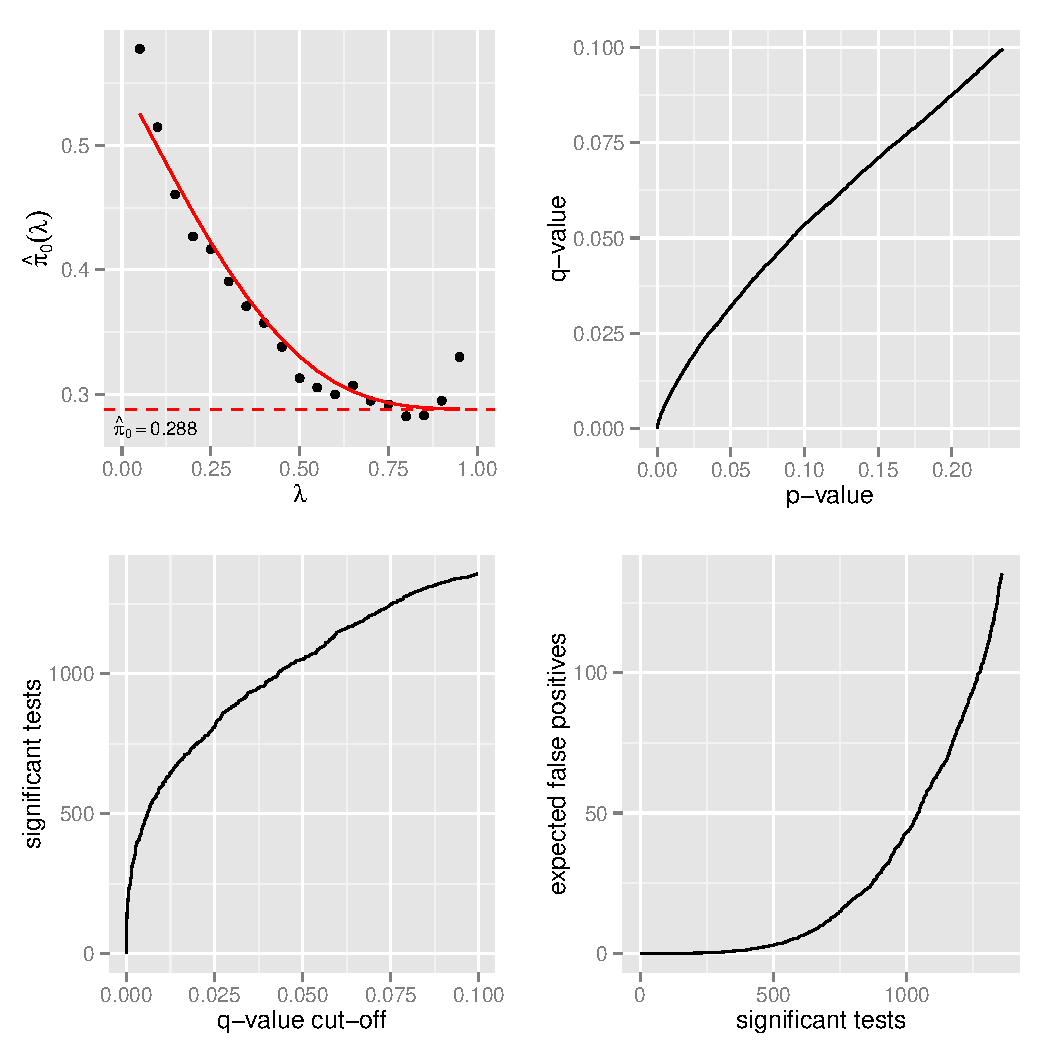
\includegraphics[width=\maxwidth]{figure/unnamed-chunk-3} 

}


\begin{kframe}\begin{alltt}
\hlkwd{summary}\hlstd{(}\hlkwd{qvalue.obj}\hlstd{(edge.odp))}
\end{alltt}
\begin{verbatim}
## 
## Call:
## qvalue(p = pval)
## 
## pi0:	0.2883	
## 
## Cumulative number of significant calls:
## 
##           <1e-04 <0.001 <0.01 <0.025 <0.05 <0.1
## p-value      184    323   594    744   903 1074
## q-value      120    246   597    812  1052 1357
## local FDR     98    173   376    514   650  832
##             <1
## p-value   2000
## q-value   2000
## local FDR 2000
\end{verbatim}
\begin{alltt}
\hlkwd{summary}\hlstd{(}\hlkwd{qvalue.obj}\hlstd{(edge.lrt))}
\end{alltt}


{\ttfamily\noindent\bfseries\color{errorcolor}{\#\# Error: error in evaluating the argument 'object' in selecting a method for function 'qvalue.obj': Error: object 'edge.lrt' not found}}\end{kframe}
\end{knitrout}

\subsection{Independent time course study: {\tt kidney} dataset}
Lets begin the analysis by importing the data and in this example use the function {\tt edgeModel} to create the models of the experiment. See {\tt ?edgeModel} for more details.

\begin{knitrout}
\definecolor{shadecolor}{rgb}{0.969, 0.969, 0.969}\color{fgcolor}\begin{kframe}
\begin{alltt}
\hlkwd{data}\hlstd{(kidney)}

\hlcom{# Interested in cortex samples }
\hlstd{sex} \hlkwb{<-} \hlstd{kidney}\hlopt{$}\hlstd{sex[kidney}\hlopt{$}\hlstd{tissue}\hlopt{==}\hlstr{"c"}\hlstd{]}
\hlstd{age} \hlkwb{<-} \hlstd{kidney}\hlopt{$}\hlstd{age[kidney}\hlopt{$}\hlstd{tissue}\hlopt{==}\hlstr{"c"}\hlstd{]}
\hlstd{kidexpr} \hlkwb{<-} \hlstd{kidney}\hlopt{$}\hlstd{kidexpr[, kidney}\hlopt{$}\hlstd{tissue}\hlopt{==}\hlstr{"c"}\hlstd{]}

\hlcom{# Create model}
\hlstd{edgeObj} \hlkwb{<-} \hlkwd{edgeModel}\hlstd{(}\hlkwc{dat}\hlstd{=kidexpr,}
                     \hlkwc{adj.var}\hlstd{=}\hlkwd{model.matrix}\hlstd{(}\hlopt{~}\hlstd{sex),}
                     \hlkwc{tme}\hlstd{=age,}
                     \hlkwc{sampling}\hlstd{=}\hlstr{"timecourse"}\hlstd{,}
                     \hlkwc{basis.df}\hlstd{=}\hlnum{4}\hlstd{)}
\end{alltt}


{\ttfamily\noindent\bfseries\color{errorcolor}{\#\# Error: could not find function "{}edgeModel"{}}}\end{kframe}
\end{knitrout}

Following similar steps in the previous example, a user can retrieve the fitted values from either statistical method in the experiment and run {\tt odp} or {\tt lrt}. 

\begin{knitrout}
\definecolor{shadecolor}{rgb}{0.969, 0.969, 0.969}\color{fgcolor}\begin{kframe}
\begin{alltt}
\hlcom{# fitted values}
\hlstd{efObject} \hlkwb{<-} \hlkwd{edgeFit}\hlstd{(edgeObj,} \hlkwc{stat.type}\hlstd{=}\hlstr{"odp"}\hlstd{)}
\hlstd{efObject} \hlkwb{<-} \hlkwd{edgeFit}\hlstd{(edgeObj,} \hlkwc{stat.type}\hlstd{=}\hlstr{"lrt"}\hlstd{)}

\hlstd{edge.odp} \hlkwb{<-} \hlkwd{odp}\hlstd{(edgeObj,} \hlkwc{bs.its}\hlstd{=}\hlnum{100}\hlstd{,} \hlkwc{verbose}\hlstd{=}\hlnum{FALSE}\hlstd{)}
\hlstd{edge.lrt} \hlkwb{<-} \hlkwd{lrt}\hlstd{(edgeObj,} \hlkwc{nullDistn}\hlstd{=}\hlstr{"bootstrap"}\hlstd{,} \hlkwc{bs.its}\hlstd{=}\hlnum{100}\hlstd{,} \hlkwc{verbose}\hlstd{=}\hlnum{FALSE}\hlstd{)}
\end{alltt}


{\ttfamily\noindent\bfseries\color{errorcolor}{\#\# Error: could not find function "{}lrtStat"{}}}\end{kframe}
\end{knitrout}

Comparing the findings between both methods:

\begin{knitrout}
\definecolor{shadecolor}{rgb}{0.969, 0.969, 0.969}\color{fgcolor}\begin{kframe}
\begin{alltt}
\hlkwd{summary}\hlstd{(}\hlkwd{qvalue.obj}\hlstd{(edge.odp))}
\end{alltt}
\begin{verbatim}
## 
## Call:
## qvalue(p = pval)
## 
## pi0:	0.3001	
## 
## Cumulative number of significant calls:
## 
##           <1e-04 <0.001 <0.01 <0.025 <0.05 <0.1
## p-value      235    387   639    779   914 1102
## q-value      204    350   649    843  1060 1372
## local FDR    164    235   427    556   662  825
##             <1
## p-value   2000
## q-value   2000
## local FDR 1880
\end{verbatim}
\begin{alltt}
\hlkwd{summary}\hlstd{(}\hlkwd{qvalue.obj}\hlstd{(edge.lrt))}
\end{alltt}


{\ttfamily\noindent\bfseries\color{errorcolor}{\#\# Error: error in evaluating the argument 'object' in selecting a method for function 'qvalue.obj': Error: object 'edge.lrt' not found}}\end{kframe}
\end{knitrout}


\subsection{Longitudinal time course study: {\tt endotoxin} dataset}
The first step is to create an {\tt ExpressionSet}:

\begin{knitrout}
\definecolor{shadecolor}{rgb}{0.969, 0.969, 0.969}\color{fgcolor}\begin{kframe}
\begin{alltt}
\hlkwd{data}\hlstd{(endotoxin)}
\hlcom{# Create ExpressionSet object}
\hlstd{expr} \hlkwb{<-} \hlstd{endotoxin}\hlopt{$}\hlstd{expr}
\hlstd{ind} \hlkwb{<-} \hlstd{endotoxin}\hlopt{$}\hlstd{individual}
\hlstd{tme} \hlkwb{<-} \hlstd{endotoxin}\hlopt{$}\hlstd{time}
\hlstd{cls} \hlkwb{<-} \hlstd{endotoxin}\hlopt{$}\hlstd{class}
\hlkwd{colnames}\hlstd{(expr)} \hlkwb{<-} \hlkwa{NULL}
\hlstd{expSet} \hlkwb{<-} \hlkwd{ExpressionSet}\hlstd{(}\hlkwc{assayData}\hlstd{=expr,}
          \hlkwc{phenoData}\hlstd{=}\hlkwd{as}\hlstd{(}\hlkwd{data.frame}\hlstd{(}\hlkwc{individual}\hlstd{=ind,} \hlkwc{time}\hlstd{=tme,} \hlkwc{class}\hlstd{=cls),}
                      \hlstr{"AnnotatedDataFrame"}\hlstd{))}
\end{alltt}
\end{kframe}
\end{knitrout}

Next step is to create an edgeSet object
\begin{knitrout}
\definecolor{shadecolor}{rgb}{0.969, 0.969, 0.969}\color{fgcolor}\begin{kframe}
\begin{alltt}
\hlstd{mNull} \hlkwb{<-} \hlopt{~-}\hlnum{1} \hlopt{+} \hlkwd{ns}\hlstd{(time,} \hlkwc{df}\hlstd{=}\hlnum{4}\hlstd{,} \hlkwc{intercept}\hlstd{=}\hlnum{FALSE}\hlstd{)}
\hlstd{mFull} \hlkwb{<-} \hlopt{~-}\hlnum{1} \hlopt{+} \hlkwd{ns}\hlstd{(time,} \hlkwc{df}\hlstd{=}\hlnum{4}\hlstd{,} \hlkwc{intercept}\hlstd{=}\hlnum{FALSE}\hlstd{)} \hlopt{+} \hlkwd{ns}\hlstd{(time,} \hlkwc{df}\hlstd{=}\hlnum{4}\hlstd{,} \hlkwc{intercept}\hlstd{=}\hlnum{FALSE}\hlstd{)}\hlopt{:}\hlstd{class} \hlopt{+} \hlstd{class}

\hlcom{# Create edgeSet object}
\hlstd{edgeObj} \hlkwb{<-} \hlkwd{edgeSet}\hlstd{(expSet,}
                   \hlkwc{full.model}\hlstd{=mFull,}
                   \hlkwc{null.model}\hlstd{=mNull,}
                   \hlkwc{individual}\hlstd{=endotoxin}\hlopt{$}\hlstd{individual)}
\end{alltt}


{\ttfamily\noindent\bfseries\color{errorcolor}{\#\# Error: could not find function "{}ns"{}}}\end{kframe}
\end{knitrout}

Determine significant genes in experiment by running {\tt odp} or {\tt lrt}.

\begin{knitrout}
\definecolor{shadecolor}{rgb}{0.969, 0.969, 0.969}\color{fgcolor}\begin{kframe}
\begin{alltt}
\hlstd{edge.odp} \hlkwb{<-} \hlkwd{odp}\hlstd{(edgeObj,} \hlkwc{bs.its}\hlstd{=}\hlnum{100}\hlstd{,} \hlkwc{verbose}\hlstd{=}\hlnum{FALSE}\hlstd{)}
\hlstd{edge.lrt} \hlkwb{<-} \hlkwd{lrt}\hlstd{(edgeObj,} \hlkwc{nullDistn}\hlstd{=}\hlstr{"bootstrap"}\hlstd{,} \hlkwc{bs.its}\hlstd{=}\hlnum{10}\hlstd{,} \hlkwc{verbose}\hlstd{=}\hlnum{FALSE}\hlstd{)}
\end{alltt}


{\ttfamily\noindent\bfseries\color{errorcolor}{\#\# Error: could not find function "{}lrtStat"{}}}\end{kframe}
\end{knitrout}

Comparing the findings between both method:

\begin{knitrout}
\definecolor{shadecolor}{rgb}{0.969, 0.969, 0.969}\color{fgcolor}\begin{kframe}
\begin{alltt}
\hlkwd{summary}\hlstd{(}\hlkwd{qvalue.obj}\hlstd{(edge.odp))}
\end{alltt}
\begin{verbatim}
## 
## Call:
## qvalue(p = pval)
## 
## pi0:	0.2753	
## 
## Cumulative number of significant calls:
## 
##           <1e-04 <0.001 <0.01 <0.025 <0.05 <0.1
## p-value      226    374   640    787   927 1105
## q-value      176    326   669    885  1108 1406
## local FDR    143    227   430    567   702  869
##             <1
## p-value   2000
## q-value   2000
## local FDR 2000
\end{verbatim}
\begin{alltt}
\hlkwd{summary}\hlstd{(}\hlkwd{qvalue.obj}\hlstd{(edge.lrt))}
\end{alltt}


{\ttfamily\noindent\bfseries\color{errorcolor}{\#\# Error: error in evaluating the argument 'object' in selecting a method for function 'qvalue.obj': Error: object 'edge.lrt' not found}}\end{kframe}
\end{knitrout}


In all three cases we notice that the optimal discovery method finds more significant genes. As shown in previous research by Storey (source), the ODP finds more significant genes for a fixed FDR when compared to the likelihood ratio test and other popular statistical methods.


\section{Features}
The \texttt{edgeSet} object inherits all methods from the \texttt{ExpressionSet} object. This makes the use of other packages written for ExprssionSet objects compatible with the edgeSet object. 

Finally, there is a method in \texttt{edge} to implement supervised normalization of microarrays on the expression matrix and the function is called \texttt{edgeSNM} which is a wrapper for the {\tt snm} packages. Also, {\tt edge} has a method {\tt edgeSVA} to create surrogate variables to reduce dependence in significance analysis.

\section*{Acknowledgements}
This software development has been supported in part by funding from the National Institutes of Health and the Office of Naval Research.

\bibliographystyle{acm}
\bibliography{edgerefs}
\end{document}
